\documentclass[a4paper,12pt]{article}
\usepackage[margin=18mm]{geometry}
\usepackage{tikz}
\usepackage{amsmath}
\newcommand{\pFourCell}[2]{\makebox[#1em][c]{\ensuremath{#2}}}
\pagestyle{empty}
\begin{document}
\section*{Spaltentreue LaTeX-Ausgabe}
\noindent Gleichung: \texttt{2*sin(sqrt((x+3)/(2+1)))=5} \hfill Zielvariable: \texttt{x} \hfill Profil: \texttt{standard}

\vspace{8mm}
\begin{center}
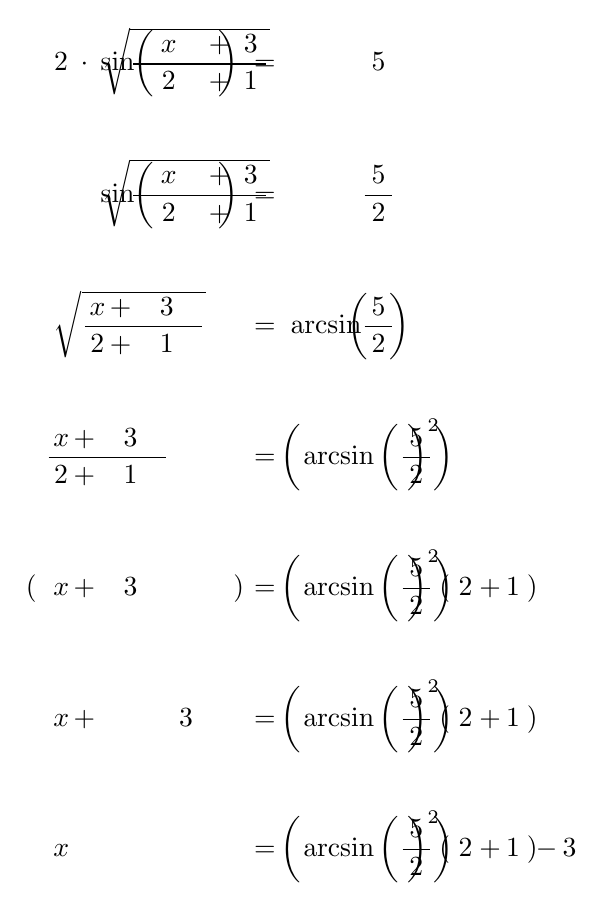
\begin{tikzpicture}[x=1em,y=-1em]
\node[anchor=base, inner sep=0pt] at (1.21,2.9) {$2$};
\node[anchor=base, inner sep=0pt] at (2.05,2.9) {$\cdot$};
\node[anchor=base, inner sep=0pt] at (5.72,2.9) {$\pFourCell{4.8}{\sqrt{\displaystyle\frac{\pFourCell{2.56}{x}\pFourCell{1.12}{+}\pFourCell{1.12}{3}}{\pFourCell{2.56}{2}\pFourCell{1.12}{+}\pFourCell{1.12}{1}}}}$};
\node[anchor=base, inner sep=0pt] at (3.25,2.9) {$\pFourCell{1.62}{\sin}$};
\node[anchor=base, inner sep=0pt] at (4.25,2.9) {$\pFourCell{0.38}{\left(\vphantom{\pFourCell{4.8}{\sqrt{\displaystyle\frac{\pFourCell{2.56}{x}\pFourCell{1.12}{+}\pFourCell{1.12}{3}}{\pFourCell{2.56}{2}\pFourCell{1.12}{+}\pFourCell{1.12}{1}}}}}\right.}$};
\node[anchor=base, inner sep=0pt] at (7.19,2.9) {$\pFourCell{0.38}{\left.\vphantom{\pFourCell{4.8}{\sqrt{\displaystyle\frac{\pFourCell{2.56}{x}\pFourCell{1.12}{+}\pFourCell{1.12}{3}}{\pFourCell{2.56}{2}\pFourCell{1.12}{+}\pFourCell{1.12}{1}}}}}\right)}$};
\node[anchor=base, inner sep=0pt] at (8.57,2.9) {$=$};
\node[anchor=base, inner sep=0pt] at (12.68,2.9) {$5$};
\node[anchor=base, inner sep=0pt] at (12.68,7.65) {$\displaystyle\frac{\pFourCell{1}{5}}{\pFourCell{1}{2}}$};
\node[anchor=base, inner sep=0pt] at (5.72,7.65) {$\pFourCell{4.8}{\sqrt{\displaystyle\frac{\pFourCell{2.56}{x}\pFourCell{1.12}{+}\pFourCell{1.12}{3}}{\pFourCell{2.56}{2}\pFourCell{1.12}{+}\pFourCell{1.12}{1}}}}$};
\node[anchor=base, inner sep=0pt] at (3.25,7.65) {$\pFourCell{1.62}{\sin}$};
\node[anchor=base, inner sep=0pt] at (4.25,7.65) {$\pFourCell{0.38}{\left(\vphantom{\pFourCell{4.8}{\sqrt{\displaystyle\frac{\pFourCell{2.56}{x}\pFourCell{1.12}{+}\pFourCell{1.12}{3}}{\pFourCell{2.56}{2}\pFourCell{1.12}{+}\pFourCell{1.12}{1}}}}}\right.}$};
\node[anchor=base, inner sep=0pt] at (7.19,7.65) {$\pFourCell{0.38}{\left.\vphantom{\pFourCell{4.8}{\sqrt{\displaystyle\frac{\pFourCell{2.56}{x}\pFourCell{1.12}{+}\pFourCell{1.12}{3}}{\pFourCell{2.56}{2}\pFourCell{1.12}{+}\pFourCell{1.12}{1}}}}}\right)}$};
\node[anchor=base, inner sep=0pt] at (8.57,7.65) {$=$};
\node[anchor=base, inner sep=0pt] at (3.69,12.4) {$\pFourCell{4.62}{\sqrt{\displaystyle\frac{\pFourCell{0.9}{x}\pFourCell{0.78}{+}\pFourCell{2.56}{3}}{\pFourCell{0.9}{2}\pFourCell{0.78}{+}\pFourCell{2.56}{1}}}}$};
\node[anchor=base, inner sep=0pt] at (8.57,12.4) {$=$};
\node[anchor=base, inner sep=0pt] at (12.68,12.4) {$\displaystyle\frac{\pFourCell{1}{5}}{\pFourCell{1}{2}}$};
\node[anchor=base, inner sep=0pt] at (10.78,12.4) {$\pFourCell{2.04}{\arcsin}$};
\node[anchor=base, inner sep=0pt] at (11.99,12.4) {$\pFourCell{0.38}{\left(\vphantom{\displaystyle\frac{\pFourCell{1}{5}}{\pFourCell{1}{2}}}\right.}$};
\node[anchor=base, inner sep=0pt] at (13.37,12.4) {$\pFourCell{0.38}{\left.\vphantom{\displaystyle\frac{\pFourCell{1}{5}}{\pFourCell{1}{2}}}\right)}$};
\node[anchor=base, inner sep=0pt] at (2.88,17.135) {$\displaystyle\frac{\pFourCell{0.9}{x}\pFourCell{0.78}{+}\pFourCell{2.56}{3}}{\pFourCell{0.9}{2}\pFourCell{0.78}{+}\pFourCell{2.56}{1}}$};
\node[anchor=base, inner sep=0pt] at (8.57,17.135) {$=$};
\node[anchor=base, inner sep=0pt] at (12.68,17.135) {$\pFourCell{1}{\arcsin\left(\displaystyle\frac{\pFourCell{1}{5}}{\pFourCell{1}{2}}\right)}$};
\node[anchor=base, inner sep=0pt] at (9.57,17.135) {$\pFourCell{0.38}{\left(\vphantom{\pFourCell{1}{\arcsin\left(\displaystyle\frac{\pFourCell{1}{5}}{\pFourCell{1}{2}}\right)}}\right.}$};
\node[anchor=base, inner sep=0pt] at (14.25,17.135) {$\pFourCell{1.38}{\left.\vphantom{\pFourCell{1}{\arcsin\left(\displaystyle\frac{\pFourCell{1}{5}}{\pFourCell{1}{2}}\right)}}\right)^{2}}$};
\node[anchor=base, inner sep=0pt] at (2.88,21.855) {$\pFourCell{0.9}{x}\pFourCell{0.78}{+}\pFourCell{2.56}{3}$};
\node[anchor=base, inner sep=0pt] at (0.19,21.855) {$\pFourCell{0.38}{\left(\vphantom{\pFourCell{0.9}{x}\pFourCell{0.78}{+}\pFourCell{2.56}{3}}\right.}$};
\node[anchor=base, inner sep=0pt] at (7.57,21.855) {$\pFourCell{0.38}{\left.\vphantom{\pFourCell{0.9}{x}\pFourCell{0.78}{+}\pFourCell{2.56}{3}}\right)}$};
\node[anchor=base, inner sep=0pt] at (8.57,21.855) {$=$};
\node[anchor=base, inner sep=0pt] at (12.68,21.855) {$\pFourCell{1}{\arcsin\left(\displaystyle\frac{\pFourCell{1}{5}}{\pFourCell{1}{2}}\right)}$};
\node[anchor=base, inner sep=0pt] at (9.57,21.855) {$\pFourCell{0.38}{\left(\vphantom{\pFourCell{1}{\arcsin\left(\displaystyle\frac{\pFourCell{1}{5}}{\pFourCell{1}{2}}\right)}}\right.}$};
\node[anchor=base, inner sep=0pt] at (14.25,21.855) {$\pFourCell{1.38}{\left.\vphantom{\pFourCell{1}{\arcsin\left(\displaystyle\frac{\pFourCell{1}{5}}{\pFourCell{1}{2}}\right)}}\right)^{2}}$};
\node[anchor=base, inner sep=0pt] at (16.65,21.855) {$\pFourCell{1}{2}\pFourCell{0.78}{+}\pFourCell{0.88}{1}$};
\node[anchor=base, inner sep=0pt] at (15.13,21.855) {$\pFourCell{0.38}{\left(\vphantom{\pFourCell{1}{2}\pFourCell{0.78}{+}\pFourCell{0.88}{1}}\right.}$};
\node[anchor=base, inner sep=0pt] at (18.17,21.855) {$\pFourCell{0.38}{\left.\vphantom{\pFourCell{1}{2}\pFourCell{0.78}{+}\pFourCell{0.88}{1}}\right)}$};
\node[anchor=base, inner sep=0pt] at (1.21,26.575) {$x$};
\node[anchor=base, inner sep=0pt] at (2.05,26.575) {$+$};
\node[anchor=base, inner sep=0pt] at (5.72,26.575) {$3$};
\node[anchor=base, inner sep=0pt] at (8.57,26.575) {$=$};
\node[anchor=base, inner sep=0pt] at (12.68,26.575) {$\pFourCell{1}{\arcsin\left(\displaystyle\frac{\pFourCell{1}{5}}{\pFourCell{1}{2}}\right)}$};
\node[anchor=base, inner sep=0pt] at (9.57,26.575) {$\pFourCell{0.38}{\left(\vphantom{\pFourCell{1}{\arcsin\left(\displaystyle\frac{\pFourCell{1}{5}}{\pFourCell{1}{2}}\right)}}\right.}$};
\node[anchor=base, inner sep=0pt] at (14.25,26.575) {$\pFourCell{1.38}{\left.\vphantom{\pFourCell{1}{\arcsin\left(\displaystyle\frac{\pFourCell{1}{5}}{\pFourCell{1}{2}}\right)}}\right)^{2}}$};
\node[anchor=base, inner sep=0pt] at (16.65,26.575) {$\pFourCell{1}{2}\pFourCell{0.78}{+}\pFourCell{0.88}{1}$};
\node[anchor=base, inner sep=0pt] at (15.13,26.575) {$\pFourCell{0.38}{\left(\vphantom{\pFourCell{1}{2}\pFourCell{0.78}{+}\pFourCell{0.88}{1}}\right.}$};
\node[anchor=base, inner sep=0pt] at (18.17,26.575) {$\pFourCell{0.38}{\left.\vphantom{\pFourCell{1}{2}\pFourCell{0.78}{+}\pFourCell{0.88}{1}}\right)}$};
\node[anchor=base, inner sep=0pt] at (1.21,31.295) {$x$};
\node[anchor=base, inner sep=0pt] at (8.57,31.295) {$=$};
\node[anchor=base, inner sep=0pt] at (12.68,31.295) {$\pFourCell{1}{\arcsin\left(\displaystyle\frac{\pFourCell{1}{5}}{\pFourCell{1}{2}}\right)}$};
\node[anchor=base, inner sep=0pt] at (9.57,31.295) {$\pFourCell{0.38}{\left(\vphantom{\pFourCell{1}{\arcsin\left(\displaystyle\frac{\pFourCell{1}{5}}{\pFourCell{1}{2}}\right)}}\right.}$};
\node[anchor=base, inner sep=0pt] at (14.25,31.295) {$\pFourCell{1.38}{\left.\vphantom{\pFourCell{1}{\arcsin\left(\displaystyle\frac{\pFourCell{1}{5}}{\pFourCell{1}{2}}\right)}}\right)^{2}}$};
\node[anchor=base, inner sep=0pt] at (16.65,31.295) {$\pFourCell{1}{2}\pFourCell{0.78}{+}\pFourCell{0.88}{1}$};
\node[anchor=base, inner sep=0pt] at (15.13,31.295) {$\pFourCell{0.38}{\left(\vphantom{\pFourCell{1}{2}\pFourCell{0.78}{+}\pFourCell{0.88}{1}}\right.}$};
\node[anchor=base, inner sep=0pt] at (18.17,31.295) {$\pFourCell{0.38}{\left.\vphantom{\pFourCell{1}{2}\pFourCell{0.78}{+}\pFourCell{0.88}{1}}\right)}$};
\node[anchor=base, inner sep=0pt] at (18.75,31.295) {$-$};
\node[anchor=base, inner sep=0pt] at (19.58,31.295) {$3$};
\end{tikzpicture}
\end{center}

\newpage
\section*{Spaltentreue LaTeX-Ausgabe mit Spaltengrenzen}
\vspace{6mm}
\begin{center}
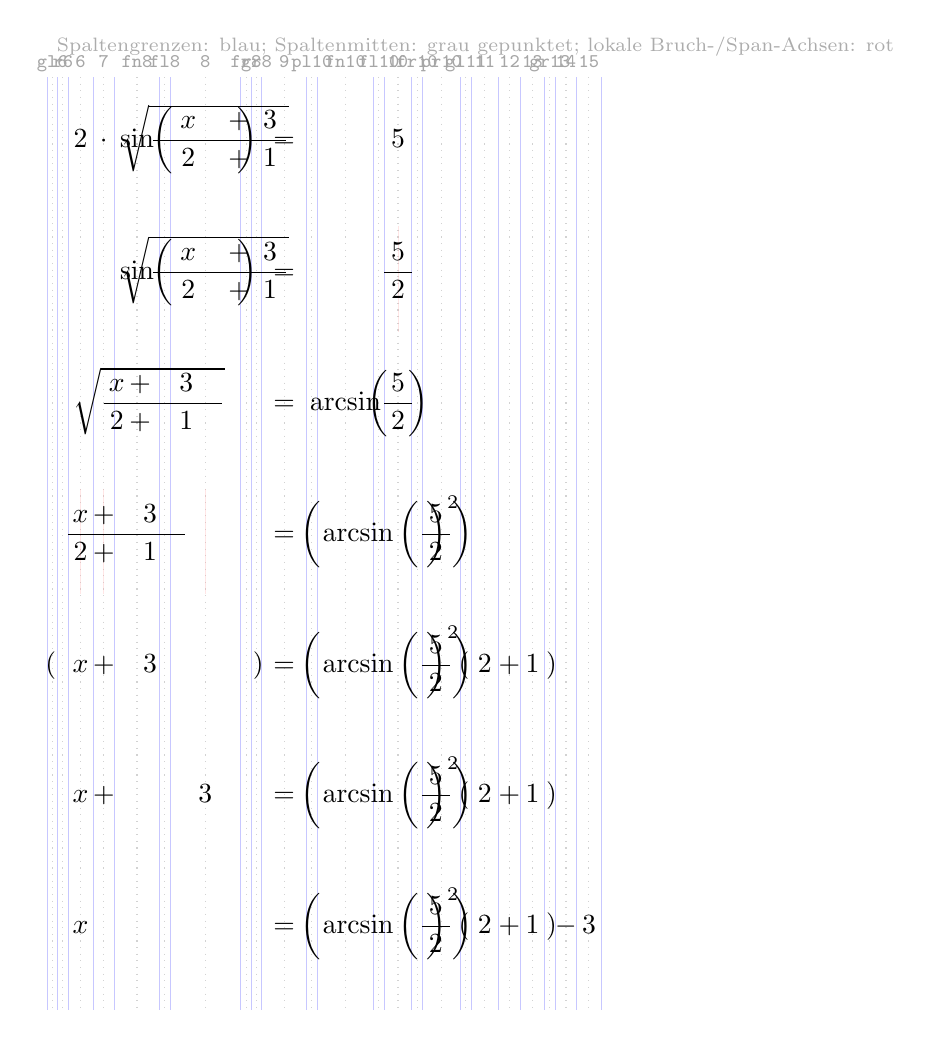
\begin{tikzpicture}[x=1em,y=-1em]
\node[font={\scriptsize}, text=gray!65, anchor=west] at (0,-0.75) {Spaltengrenzen: blau; Spaltenmitten: grau gepunktet; lokale Bruch-/Span-Achsen: rot};
\draw[blue!22, line width=0.28pt] (0,0.35) -- (0,34.08);
\draw[blue!22, line width=0.28pt] (0.38,0.35) -- (0.38,34.08);
\draw[blue!22, line width=0.28pt] (0.76,0.35) -- (0.76,34.08);
\draw[blue!22, line width=0.28pt] (1.66,0.35) -- (1.66,34.08);
\draw[blue!22, line width=0.28pt] (2.44,0.35) -- (2.44,34.08);
\draw[blue!22, line width=0.28pt] (4.06,0.35) -- (4.06,34.08);
\draw[blue!22, line width=0.28pt] (4.44,0.35) -- (4.44,34.08);
\draw[blue!22, line width=0.28pt] (7,0.35) -- (7,34.08);
\draw[blue!22, line width=0.28pt] (7.38,0.35) -- (7.38,34.08);
\draw[blue!22, line width=0.28pt] (7.76,0.35) -- (7.76,34.08);
\draw[blue!22, line width=0.28pt] (9.38,0.35) -- (9.38,34.08);
\draw[blue!22, line width=0.28pt] (9.76,0.35) -- (9.76,34.08);
\draw[blue!22, line width=0.28pt] (11.8,0.35) -- (11.8,34.08);
\draw[blue!22, line width=0.28pt] (12.18,0.35) -- (12.18,34.08);
\draw[blue!22, line width=0.28pt] (13.18,0.35) -- (13.18,34.08);
\draw[blue!22, line width=0.28pt] (13.56,0.35) -- (13.56,34.08);
\draw[blue!22, line width=0.28pt] (14.94,0.35) -- (14.94,34.08);
\draw[blue!22, line width=0.28pt] (15.32,0.35) -- (15.32,34.08);
\draw[blue!22, line width=0.28pt] (16.32,0.35) -- (16.32,34.08);
\draw[blue!22, line width=0.28pt] (17.1,0.35) -- (17.1,34.08);
\draw[blue!22, line width=0.28pt] (17.98,0.35) -- (17.98,34.08);
\draw[blue!22, line width=0.28pt] (18.36,0.35) -- (18.36,34.08);
\draw[blue!22, line width=0.28pt] (19.14,0.35) -- (19.14,34.08);
\draw[blue!22, line width=0.28pt] (20.02,0.35) -- (20.02,34.08);
\draw[gray!35, dotted] (0.19,0.35) -- (0.19,34.08);
\node[font={\ttfamily\scriptsize}, text=gray!70, anchor=base] at (0.19,0) {gl6};
\draw[gray!35, dotted] (0.57,0.35) -- (0.57,34.08);
\node[font={\ttfamily\scriptsize}, text=gray!70, anchor=base] at (0.57,0) {r6};
\draw[gray!35, dotted] (1.21,0.35) -- (1.21,34.08);
\node[font={\ttfamily\scriptsize}, text=gray!70, anchor=base] at (1.21,0) {6};
\draw[gray!35, dotted] (2.05,0.35) -- (2.05,34.08);
\node[font={\ttfamily\scriptsize}, text=gray!70, anchor=base] at (2.05,0) {7};
\draw[gray!35, dotted] (3.25,0.35) -- (3.25,34.08);
\node[font={\ttfamily\scriptsize}, text=gray!70, anchor=base] at (3.25,0) {fn8};
\draw[gray!35, dotted] (4.25,0.35) -- (4.25,34.08);
\node[font={\ttfamily\scriptsize}, text=gray!70, anchor=base] at (4.25,0) {fl8};
\draw[gray!35, dotted] (5.72,0.35) -- (5.72,34.08);
\node[font={\ttfamily\scriptsize}, text=gray!70, anchor=base] at (5.72,0) {8};
\draw[gray!35, dotted] (7.19,0.35) -- (7.19,34.08);
\node[font={\ttfamily\scriptsize}, text=gray!70, anchor=base] at (7.19,0) {fr8};
\draw[gray!35, dotted] (7.57,0.35) -- (7.57,34.08);
\node[font={\ttfamily\scriptsize}, text=gray!70, anchor=base] at (7.57,0) {gr8};
\draw[gray!35, dotted] (8.57,0.35) -- (8.57,34.08);
\node[font={\ttfamily\scriptsize}, text=gray!70, anchor=base] at (8.57,0) {9};
\draw[gray!35, dotted] (9.57,0.35) -- (9.57,34.08);
\node[font={\ttfamily\scriptsize}, text=gray!70, anchor=base] at (9.57,0) {pl10};
\draw[gray!35, dotted] (10.78,0.35) -- (10.78,34.08);
\node[font={\ttfamily\scriptsize}, text=gray!70, anchor=base] at (10.78,0) {fn10};
\draw[gray!35, dotted] (11.99,0.35) -- (11.99,34.08);
\node[font={\ttfamily\scriptsize}, text=gray!70, anchor=base] at (11.99,0) {fl10};
\draw[gray!35, dotted] (12.68,0.35) -- (12.68,34.08);
\node[font={\ttfamily\scriptsize}, text=gray!70, anchor=base] at (12.68,0) {10};
\draw[gray!35, dotted] (13.37,0.35) -- (13.37,34.08);
\node[font={\ttfamily\scriptsize}, text=gray!70, anchor=base] at (13.37,0) {fr10};
\draw[gray!35, dotted] (14.25,0.35) -- (14.25,34.08);
\node[font={\ttfamily\scriptsize}, text=gray!70, anchor=base] at (14.25,0) {pr10};
\draw[gray!35, dotted] (15.13,0.35) -- (15.13,34.08);
\node[font={\ttfamily\scriptsize}, text=gray!70, anchor=base] at (15.13,0) {gl11};
\draw[gray!35, dotted] (15.82,0.35) -- (15.82,34.08);
\node[font={\ttfamily\scriptsize}, text=gray!70, anchor=base] at (15.82,0) {11};
\draw[gray!35, dotted] (16.71,0.35) -- (16.71,34.08);
\node[font={\ttfamily\scriptsize}, text=gray!70, anchor=base] at (16.71,0) {12};
\draw[gray!35, dotted] (17.54,0.35) -- (17.54,34.08);
\node[font={\ttfamily\scriptsize}, text=gray!70, anchor=base] at (17.54,0) {13};
\draw[gray!35, dotted] (18.17,0.35) -- (18.17,34.08);
\node[font={\ttfamily\scriptsize}, text=gray!70, anchor=base] at (18.17,0) {gr13};
\draw[gray!35, dotted] (18.75,0.35) -- (18.75,34.08);
\node[font={\ttfamily\scriptsize}, text=gray!70, anchor=base] at (18.75,0) {14};
\draw[gray!35, dotted] (19.58,0.35) -- (19.58,34.08);
\node[font={\ttfamily\scriptsize}, text=gray!70, anchor=base] at (19.58,0) {15};
\node[anchor=base, inner sep=0pt] at (1.21,2.9) {$2$};
\node[anchor=base, inner sep=0pt] at (2.05,2.9) {$\cdot$};
\node[anchor=base, inner sep=0pt] at (5.72,2.9) {$\pFourCell{4.8}{\sqrt{\displaystyle\frac{\pFourCell{2.56}{x}\pFourCell{1.12}{+}\pFourCell{1.12}{3}}{\pFourCell{2.56}{2}\pFourCell{1.12}{+}\pFourCell{1.12}{1}}}}$};
\node[anchor=base, inner sep=0pt] at (3.25,2.9) {$\pFourCell{1.62}{\sin}$};
\node[anchor=base, inner sep=0pt] at (4.25,2.9) {$\pFourCell{0.38}{\left(\vphantom{\pFourCell{4.8}{\sqrt{\displaystyle\frac{\pFourCell{2.56}{x}\pFourCell{1.12}{+}\pFourCell{1.12}{3}}{\pFourCell{2.56}{2}\pFourCell{1.12}{+}\pFourCell{1.12}{1}}}}}\right.}$};
\node[anchor=base, inner sep=0pt] at (7.19,2.9) {$\pFourCell{0.38}{\left.\vphantom{\pFourCell{4.8}{\sqrt{\displaystyle\frac{\pFourCell{2.56}{x}\pFourCell{1.12}{+}\pFourCell{1.12}{3}}{\pFourCell{2.56}{2}\pFourCell{1.12}{+}\pFourCell{1.12}{1}}}}}\right)}$};
\node[anchor=base, inner sep=0pt] at (8.57,2.9) {$=$};
\node[anchor=base, inner sep=0pt] at (12.68,2.9) {$5$};
\draw[red!30, opacity=0.32, line width=0.35pt] (12.68,5.75) -- (12.68,9.55);
\node[anchor=base, inner sep=0pt] at (12.68,7.65) {$\displaystyle\frac{\pFourCell{1}{5}}{\pFourCell{1}{2}}$};
\node[anchor=base, inner sep=0pt] at (5.72,7.65) {$\pFourCell{4.8}{\sqrt{\displaystyle\frac{\pFourCell{2.56}{x}\pFourCell{1.12}{+}\pFourCell{1.12}{3}}{\pFourCell{2.56}{2}\pFourCell{1.12}{+}\pFourCell{1.12}{1}}}}$};
\node[anchor=base, inner sep=0pt] at (3.25,7.65) {$\pFourCell{1.62}{\sin}$};
\node[anchor=base, inner sep=0pt] at (4.25,7.65) {$\pFourCell{0.38}{\left(\vphantom{\pFourCell{4.8}{\sqrt{\displaystyle\frac{\pFourCell{2.56}{x}\pFourCell{1.12}{+}\pFourCell{1.12}{3}}{\pFourCell{2.56}{2}\pFourCell{1.12}{+}\pFourCell{1.12}{1}}}}}\right.}$};
\node[anchor=base, inner sep=0pt] at (7.19,7.65) {$\pFourCell{0.38}{\left.\vphantom{\pFourCell{4.8}{\sqrt{\displaystyle\frac{\pFourCell{2.56}{x}\pFourCell{1.12}{+}\pFourCell{1.12}{3}}{\pFourCell{2.56}{2}\pFourCell{1.12}{+}\pFourCell{1.12}{1}}}}}\right)}$};
\node[anchor=base, inner sep=0pt] at (8.57,7.65) {$=$};
\node[anchor=base, inner sep=0pt] at (3.69,12.4) {$\pFourCell{4.62}{\sqrt{\displaystyle\frac{\pFourCell{0.9}{x}\pFourCell{0.78}{+}\pFourCell{2.56}{3}}{\pFourCell{0.9}{2}\pFourCell{0.78}{+}\pFourCell{2.56}{1}}}}$};
\node[anchor=base, inner sep=0pt] at (8.57,12.4) {$=$};
\node[anchor=base, inner sep=0pt] at (12.68,12.4) {$\displaystyle\frac{\pFourCell{1}{5}}{\pFourCell{1}{2}}$};
\node[anchor=base, inner sep=0pt] at (10.78,12.4) {$\pFourCell{2.04}{\arcsin}$};
\node[anchor=base, inner sep=0pt] at (11.99,12.4) {$\pFourCell{0.38}{\left(\vphantom{\displaystyle\frac{\pFourCell{1}{5}}{\pFourCell{1}{2}}}\right.}$};
\node[anchor=base, inner sep=0pt] at (13.37,12.4) {$\pFourCell{0.38}{\left.\vphantom{\displaystyle\frac{\pFourCell{1}{5}}{\pFourCell{1}{2}}}\right)}$};
\draw[red!30, opacity=0.32, line width=0.35pt] (1.21,15.25) -- (1.21,19.02);
\draw[red!30, opacity=0.32, line width=0.35pt] (2.05,15.25) -- (2.05,19.02);
\draw[red!30, opacity=0.32, line width=0.35pt] (5.72,15.25) -- (5.72,19.02);
\node[anchor=base, inner sep=0pt] at (2.88,17.135) {$\displaystyle\frac{\pFourCell{0.9}{x}\pFourCell{0.78}{+}\pFourCell{2.56}{3}}{\pFourCell{0.9}{2}\pFourCell{0.78}{+}\pFourCell{2.56}{1}}$};
\node[anchor=base, inner sep=0pt] at (8.57,17.135) {$=$};
\node[anchor=base, inner sep=0pt] at (12.68,17.135) {$\pFourCell{1}{\arcsin\left(\displaystyle\frac{\pFourCell{1}{5}}{\pFourCell{1}{2}}\right)}$};
\node[anchor=base, inner sep=0pt] at (9.57,17.135) {$\pFourCell{0.38}{\left(\vphantom{\pFourCell{1}{\arcsin\left(\displaystyle\frac{\pFourCell{1}{5}}{\pFourCell{1}{2}}\right)}}\right.}$};
\node[anchor=base, inner sep=0pt] at (14.25,17.135) {$\pFourCell{1.38}{\left.\vphantom{\pFourCell{1}{\arcsin\left(\displaystyle\frac{\pFourCell{1}{5}}{\pFourCell{1}{2}}\right)}}\right)^{2}}$};
\node[anchor=base, inner sep=0pt] at (2.88,21.855) {$\pFourCell{0.9}{x}\pFourCell{0.78}{+}\pFourCell{2.56}{3}$};
\node[anchor=base, inner sep=0pt] at (0.19,21.855) {$\pFourCell{0.38}{\left(\vphantom{\pFourCell{0.9}{x}\pFourCell{0.78}{+}\pFourCell{2.56}{3}}\right.}$};
\node[anchor=base, inner sep=0pt] at (7.57,21.855) {$\pFourCell{0.38}{\left.\vphantom{\pFourCell{0.9}{x}\pFourCell{0.78}{+}\pFourCell{2.56}{3}}\right)}$};
\node[anchor=base, inner sep=0pt] at (8.57,21.855) {$=$};
\node[anchor=base, inner sep=0pt] at (12.68,21.855) {$\pFourCell{1}{\arcsin\left(\displaystyle\frac{\pFourCell{1}{5}}{\pFourCell{1}{2}}\right)}$};
\node[anchor=base, inner sep=0pt] at (9.57,21.855) {$\pFourCell{0.38}{\left(\vphantom{\pFourCell{1}{\arcsin\left(\displaystyle\frac{\pFourCell{1}{5}}{\pFourCell{1}{2}}\right)}}\right.}$};
\node[anchor=base, inner sep=0pt] at (14.25,21.855) {$\pFourCell{1.38}{\left.\vphantom{\pFourCell{1}{\arcsin\left(\displaystyle\frac{\pFourCell{1}{5}}{\pFourCell{1}{2}}\right)}}\right)^{2}}$};
\node[anchor=base, inner sep=0pt] at (16.65,21.855) {$\pFourCell{1}{2}\pFourCell{0.78}{+}\pFourCell{0.88}{1}$};
\node[anchor=base, inner sep=0pt] at (15.13,21.855) {$\pFourCell{0.38}{\left(\vphantom{\pFourCell{1}{2}\pFourCell{0.78}{+}\pFourCell{0.88}{1}}\right.}$};
\node[anchor=base, inner sep=0pt] at (18.17,21.855) {$\pFourCell{0.38}{\left.\vphantom{\pFourCell{1}{2}\pFourCell{0.78}{+}\pFourCell{0.88}{1}}\right)}$};
\node[anchor=base, inner sep=0pt] at (1.21,26.575) {$x$};
\node[anchor=base, inner sep=0pt] at (2.05,26.575) {$+$};
\node[anchor=base, inner sep=0pt] at (5.72,26.575) {$3$};
\node[anchor=base, inner sep=0pt] at (8.57,26.575) {$=$};
\node[anchor=base, inner sep=0pt] at (12.68,26.575) {$\pFourCell{1}{\arcsin\left(\displaystyle\frac{\pFourCell{1}{5}}{\pFourCell{1}{2}}\right)}$};
\node[anchor=base, inner sep=0pt] at (9.57,26.575) {$\pFourCell{0.38}{\left(\vphantom{\pFourCell{1}{\arcsin\left(\displaystyle\frac{\pFourCell{1}{5}}{\pFourCell{1}{2}}\right)}}\right.}$};
\node[anchor=base, inner sep=0pt] at (14.25,26.575) {$\pFourCell{1.38}{\left.\vphantom{\pFourCell{1}{\arcsin\left(\displaystyle\frac{\pFourCell{1}{5}}{\pFourCell{1}{2}}\right)}}\right)^{2}}$};
\node[anchor=base, inner sep=0pt] at (16.65,26.575) {$\pFourCell{1}{2}\pFourCell{0.78}{+}\pFourCell{0.88}{1}$};
\node[anchor=base, inner sep=0pt] at (15.13,26.575) {$\pFourCell{0.38}{\left(\vphantom{\pFourCell{1}{2}\pFourCell{0.78}{+}\pFourCell{0.88}{1}}\right.}$};
\node[anchor=base, inner sep=0pt] at (18.17,26.575) {$\pFourCell{0.38}{\left.\vphantom{\pFourCell{1}{2}\pFourCell{0.78}{+}\pFourCell{0.88}{1}}\right)}$};
\node[anchor=base, inner sep=0pt] at (1.21,31.295) {$x$};
\node[anchor=base, inner sep=0pt] at (8.57,31.295) {$=$};
\node[anchor=base, inner sep=0pt] at (12.68,31.295) {$\pFourCell{1}{\arcsin\left(\displaystyle\frac{\pFourCell{1}{5}}{\pFourCell{1}{2}}\right)}$};
\node[anchor=base, inner sep=0pt] at (9.57,31.295) {$\pFourCell{0.38}{\left(\vphantom{\pFourCell{1}{\arcsin\left(\displaystyle\frac{\pFourCell{1}{5}}{\pFourCell{1}{2}}\right)}}\right.}$};
\node[anchor=base, inner sep=0pt] at (14.25,31.295) {$\pFourCell{1.38}{\left.\vphantom{\pFourCell{1}{\arcsin\left(\displaystyle\frac{\pFourCell{1}{5}}{\pFourCell{1}{2}}\right)}}\right)^{2}}$};
\node[anchor=base, inner sep=0pt] at (16.65,31.295) {$\pFourCell{1}{2}\pFourCell{0.78}{+}\pFourCell{0.88}{1}$};
\node[anchor=base, inner sep=0pt] at (15.13,31.295) {$\pFourCell{0.38}{\left(\vphantom{\pFourCell{1}{2}\pFourCell{0.78}{+}\pFourCell{0.88}{1}}\right.}$};
\node[anchor=base, inner sep=0pt] at (18.17,31.295) {$\pFourCell{0.38}{\left.\vphantom{\pFourCell{1}{2}\pFourCell{0.78}{+}\pFourCell{0.88}{1}}\right)}$};
\node[anchor=base, inner sep=0pt] at (18.75,31.295) {$-$};
\node[anchor=base, inner sep=0pt] at (19.58,31.295) {$3$};
\end{tikzpicture}
\end{center}
\end{document}
